%!TEX root = ../authorinstr.tex

\section{Introduction}

Designing an optimal controller for a given environment and goal can be a complex task. Reinforcement Learning (RL) techniques exist to address these tasks by learning a policy that results in choosing optimal actions in a given state. This way agents are able to learn complex behaviour, such as playing backgammon \cite{tesauro2002programming} or chess \cite{baxter1999knightcap},
real life quadripedal walking \cite{kohl2004policy}, or autonomous simulated driving \cite{}. \\  %%ADD ALPHAGO


In initial stages the agent performs random action, while learning to approximate received reward after the chosen actions. This should enable the agent to learn an optimal policy for the defined reward function. For this learning process multiple techniques exist. In our work we will compare the performance of a recently published techniques, Neural Fitted Actor Critic (NFAC), with two older techniques, SARSA and CACLA, in two environments.

Recently new environment have arisen for agents to engage in, such as OpenAI \cite{REFERENCE}. Here multiple environments are presented, such as playing Atari games and more classic problems as MountainCar and CartPole. In our work we chose to use continueos variants of MountainCar and LunarLander, see figure \ref{fig:mountainlunar}, where both the action and state spaces are continues. 
Discrete state spaces are known to work well with RL-techniques, although continueus state-spaces present themselves often more of a challenge \cite{TODO}. \\

%\subsection*{SARSA}
In \cite{nichols2015continuous}, Nichols e.a. describe an approach of using SARSA, together with a technique based on Newtons Method (NM) to obtain continueos action selection. 
In our work we will use SARSA in a similar way. Instead of using NM for continuous action selection, we will use Gradient Descend (GD) to obtain actions resulting in a higher expected Q-value.

%\subsection*{CALCA}
%%TODO shortly describe prev work CACLA
%\subsection*{NFAC}
%%TODO shorty describe prev work NFAC





%Furthermore the required level
%of discritization can not be known in all 11 cases, and having to discover it is time intensive \cite{van2007reinforcement}. %citatie naar de cacla paper
%This potential problem can be solved by keeping the state and action space continuous in the environment representation of the agent. \\
%Several new reinforcement learning algorithms and adaptations of existing reinforcement algorithms were developed to model continuous
%state and action spaces. In this paper we will benchamark one such algorithm, named Neural Fitted Actor Critic (NFAC), which was develeped in August 2016 \cite{zimmer2016neural}
%against two established (at the time of the writing of this paper) continuous reinforcement learning algorithms, named CACLA (Continuous Actor Critic Learning Automaton)
%\cite{van2007reinforcement}
%and SARSA (State Action Reward State Action) adapted for continuous state- and action-spaces \cite{nichols2014application} with gradient descent (referred to in this paper as GD-SARSA). \\
First a formal background will be given on connectionist reinforcement learning with the use of MLP's as function approximators,
and on extending this to continuous state- and action-spaces. In the methods section the three algorithms that are compared
 in this paper the implementation of these algorithms are explained in detail. After that setup of the experiments will be discussed.
Finally the results will be presented and evaluated, and the final conclusions will be drawn regarding NFAC compared to CACLA and GD-SARSA.

\begin{figure}[t]
 \centering 
    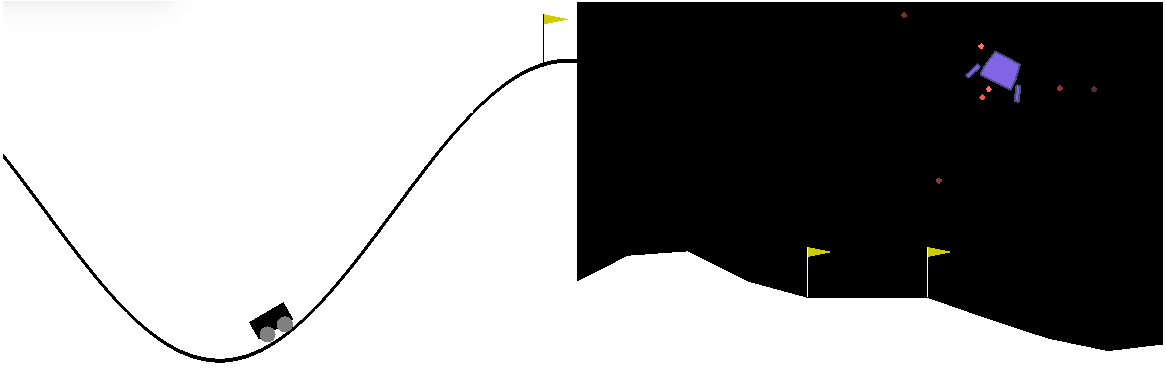
\includegraphics[width = 0.7\columnwidth]{figs/mountainlunar.png}
 \caption{Left: MountainCar Environment, Right: LunarLander Environment.}
\label{fig:mountainlunar}
\end{figure}
